\begin{usecase}{Manage Scheduling Conflicts}
  \ucbasicinfo{Medium}{Regular}
  \ucshortdescription{This UC allows the user to manage scheduling conflicts by suggesting resolutions when overlapping events are detected.}
  \uctrigger{This UC is triggered when an automatically added event overlaps with an existing event.}
  \ucactors{User}{None}
  \ucpreconditions{
    \begin{itemize}
      \item User is logged in.
      \item Conflicting events list is not empty.
    \end{itemize}
  }
  \ucrelationships{N/A}{N/A}{N/A}
  \ucinputsoutputs{
    \begin{itemize}
      \item \textbf{Conflicting events} (Source: System)
      \item \textbf{Event to override} (Source: User)
    \end{itemize}
  }{
    \begin{itemize}
      \item \textbf{Conflict resolution suggestion} (Destination: User Interface)
      \item \textbf{Updated event schedules} (Destination: Calendar)
    \end{itemize}
  }
  \ucmainflow{
    \begin{enumerate}
      \item The user opens the application and clicks on the view conflicts icon
            \ucinfo{The application shows all the conflics with their resolution options}
      \item The user chooses the best fit option to manage each conflict
            \ucinfo{The conflict is resolved and is removed from the conflict list }

    \end{enumerate}
  }
  \ucalternateflows{
    \begin{enumerate}
      \item If the user doesn't choose any option, it shows conflicting status until the user chooses any option or the event expires.
      \item If the user clicks on reject the event is left overlapping.
    \end{enumerate}
  }
  \ucexceptions{
    \begin{itemize}
      \item Network failure
    \end{itemize}
  }
  \ucconclusion{The UC ends when the conflicting events are either resolved or marked as conflicting, based on the user's choice.}
  \ucpostconditions{The calendar reflects the user's decision regarding event conflicts.}
  \ucspecialrequirements{The system should provide best suggestions for resolving conflicts.}
\end{usecase}

\begin{figure}[!h]
  \centering
  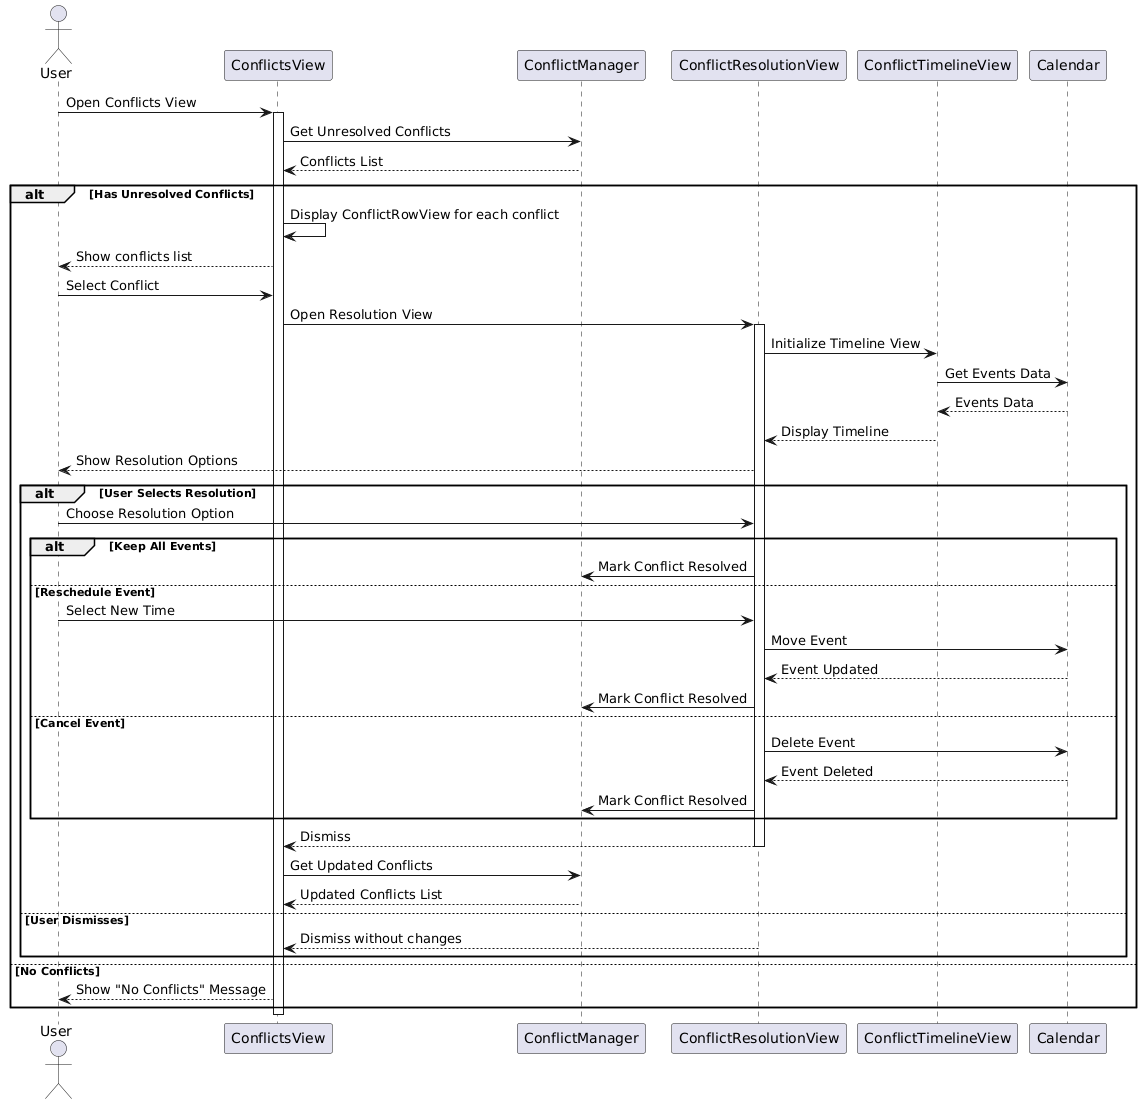
\includegraphics[width=\textwidth]{images/docs/diagrams/sequence-diagrams/all-sequence-diagrams/Manage Scheduling Conflicts.png}
  \caption{Manage Scheduling Conflicts Sequence Diagram}
  \label{fig:seq/manage-scheduling-conflicts}
\end{figure}

The ``Manage Scheduling Conflicts Sequence Diagram'', shown in \textbf{Figure~\ref{fig:seq/manage-scheduling-conflicts}}, illustrates the interactive process of handling calendar conflicts within Jadwal. The sequence begins with the ViewConflicts gRPC call, where the user requests to see existing scheduling conflicts.

The Backend processes this request through several steps:
\begin{enumerate}
  \item Retrieves the list of conflicts from the Database via FetchConflicts
  \item Generates intelligent resolution options for each conflict
  \item Returns the conflicts and their possible resolutions to the user
\end{enumerate}

When the user selects a resolution option, the process continues with:
\begin{itemize}
  \item The ResolveConflict gRPC call carrying the user's selected option
  \item Database update to reflect the chosen resolution
  \item Retrieval of relevant device IDs for notification purposes
  \item Push notification dispatch through Apple Push Notification service (APNs) to inform affected users
\end{itemize}

If the user chooses to reject resolution, the system maintains the conflict status without further action. This workflow ensures users have complete control over their schedule while maintaining awareness of conflicts through push notifications. The system's ability to generate and present resolution options helps users make informed decisions about their scheduling conflicts.